% Created 2019-01-30 Wed 22:14
\documentclass[11pt]{article}
\usepackage[utf8]{inputenc}
\usepackage[T1]{fontenc}
\usepackage{fixltx2e}
\usepackage{graphicx}
\usepackage{longtable}
\usepackage{float}
\usepackage{wrapfig}
\usepackage{rotating}
\usepackage[normalem]{ulem}
\usepackage{amsmath}
\usepackage{textcomp}
\usepackage{marvosym}
\usepackage{wasysym}
\usepackage{amssymb}
\usepackage{hyperref}
\tolerance=1000
\usepackage{minted}
\usepackage{amsthm}
\usepackage[margin=1.0in]{geometry}
\setlength{\parindent}{0pt}
\setlength{\parskip}{\baselineskip}
\author{Thomas Alford}
\date{\today}
\title{Ph21 Problem Set 2}
\hypersetup{
  pdfkeywords={},
  pdfsubject={},
  pdfcreator={Emacs 25.2.1 (Org mode 8.2.10)}}
\begin{document}

\maketitle

\section*{Mathematical Introduction- Part I}
\label{sec-1}
\subsection*{1}
\label{sec-1-1}
If we set $h(x) = \delta(x - x_0)$, we have $h(x) = \sum _{k=-\infty }^{\infty}
\frac{1}{L} e^{-2 \pi i x f_k} \left(\int_0^L \delta \left(x-x_0\right) e^{2 \pi i x
f_k} \, dx\right)}$.

Using the sifting theorem for the delta function, the right side is equivalent
to $$\sum _{k=-\infty }^{\infty } \frac{1}{L} e^{2 \pi i x_0 f_k} e^{-2 \pi i x
f_k}$$.

$$ = \sum _{k=-\infty }^{\infty } \frac{1}{L} e^{2 \pi  i x_0 f_k} e^{-2 \pi  i x f_k}$$

$$ = \sum _{k=-\infty }^{\infty } \frac{1}{L} e^{-2 \pi  i \left(x-x_0\right) f_k}$$

Now, we'll assume that each partition is small enough that we can evaluate this
sum as an integral, and so we obtain

$$\frac{1}{L} \int_{-\infty }^{\infty } e^{-\frac{2 \pi i k
\left(x-x_0\right)}{L}} \, dk$$

Now, we have the formula $\delta (x-a)=\frac{1}{2 \pi}\int_{-\infty }^{\infty } e^{i p
(x-a)} \, dp}$. Using this, we obtain

$$ = \frac{1}{L} (2 \pi ) \frac{1}{2 \pi } L  \delta\left(x-x_0\right)}$$

$$ = \delta(x - x_0)$$

So this result is indeed consistent, at least for h(x) as a delta function.


\subsection*{2}
\label{sec-1-2}
Here we start out with the complex linear combination of exponentials:
$$(a+i b) e^{-\frac{2 \pi  i x}{L}}+(a-i b) e^{\frac{2 \pi  i x}{L}}$$

Expanding this out in terms of trig function, we obtain 
$$2 a \cos \left(\frac{2 \pi  x}{L}\right)+2 b \sin \left(\frac{2 \pi  x}{L}\right)$$

Now, setting $a = \frac{1}{2} A \sin (\varphi )$ and $b = \frac{1}{2} A \cos
(\varphi )$, we obtain through the sine sum formula 

$$A \sin (\frac{2 \pi x}{L} + \varphi)$$. Thus, we can create any generic sine
function with given frequency out of the two fourier terms of the given
frequency.

\subsection*{3}
\label{sec-1-3}
Here we have that $e^{\frac{2 \pi i x f_k}{L}} = \cos(\frac{2 \pi i x
f_k}{L}) + i \sin(\frac{2 \pi i x f_k}{L})$.

$$ = \cos(\frac{2 \pi i x f_k}{L}) + i \sin(\frac{2 \pi i x f_k}{L})$$

Additionally, $$e^{\frac{-2 \pi i x f_k}{L}} = \cos(\frac{2 \pi i x f_k}{L}) -
i \sin(\frac{2 \pi i x f_k}{L})$$.

Thus, we see that the real parts of these expressions are the same, and the
imaginary parts differ by a negative sign. Looking at the expression for the
Fourier coefficients, $\tilde{h_k} = \frac{1}{L} \int_0^L h(x) e^{\frac{2 \pi i
x f_k}{L}}$, we have that if h(x) is real, then we have that $\tilde{h}_{-k} =
\tilde{h}_k$.

\subsection*{4}
\label{sec-1-4}
Here we have that H(x) = h$^{\text{(1)}}$(x) h$^{\text{(2)}}$(x).

So, $\tilde{H}_k=\left(\sum _{k=-\infty }^{\infty } \tilde{h}^1{}_k e^{-\frac{2
\pi i k x}{L}}\right) \sum _{k=-\infty }^{\infty } \tilde{h}^2{}_k e^{-\frac{2
\pi i k x}{L}}$.

Expanding out over values of k, for each e-term we get coefficients multiplied
of all the different ways to add up to k. This can be any combination of (k',
k - k'), where k' goes from -$\infty$ to +$\infty$, since k runs from -$\infty$ to
+$\infty$.

Thus, we simply obtain $$\sum _{k'=-\infty }^{\infty } e^{-\frac{2 \pi i k
x}{L}} \tilde{h}^2{}_{k-k'} \tilde{h}^1{}_{k'}$$.

For the next part, if we try obtaining a coefficients for generic k, we get for
$k'\neq 10$, $\tilde{h}^1{}_{k-k'} \tilde{h}^2{}_{k'} = 0$ due to $h^{(2)}$'s
unit pulse coefficients centered around 10. If $k' = 10$, we get
$\tilde{h}^{(1)}_{k-10}$. So, we're effectively just shifting all the Fourier
coefficeints of the smooth function centered at 0 over by 10, giving us a
smooth function centered at 10 for the Fourier coefficients of $\tilde{H}(x)$.

For example, let's say $h^{(1)}(x) = x^2$ and plot H.

\begin{minted}[frame=lines,fontsize=\scriptsize]{python}
X = np.linspace(-30, 30, 1000)
plt.figure(figsize=(10, 5))
plt.plot(X, X ** 2, label = 'h1_k')
plt.plot(X, (X - 10) ** 2, label='H_k')
plt.legend()
plt.grid(True)
plt.xlabel('k')
plt.xlim([-20, 30])
plt.ylabel('Fourier Coefficient')
plt.title('Comparing Fourier Coefficients with a Delta Function Convolution')
plt.show()
\end{minted}

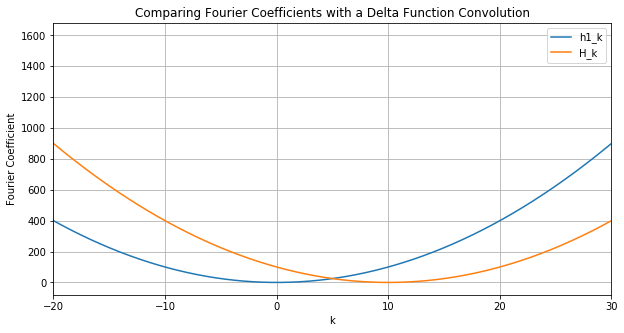
\includegraphics[width=.9\linewidth]{./obipy-resources/17087KBx.png}


\subsection*{5}
\label{sec-1-5}

We'll create a cosine function $C + A cos(2 \pi f t + \phi)$, with $f = f_k =
\frac{k}{L}$, with $L = 10, k = 5, C = 2, A = 3, \phi = \frac{\pi}{2}$.

\begin{minted}[frame=lines,fontsize=\scriptsize]{python}
from astropy.io.votable import parse
import numpy as np
import scipy
from scipy.signal import lombscargle
import matplotlib.pyplot as plt
%matplotlib inline
\end{minted}


\begin{minted}[frame=lines,fontsize=\scriptsize]{python}
def cosine(t, C, A, k, L, phi):
    return C + A * np.cos(2 * np.pi * (k / L) * t + phi)

# here we'll set C = 2, A = 3, k = 5, L = 10, phi = pi/8
X = np.linspace(0, 10, 10000)
Y = cosine(X, 2., 3., 5., 10., np.pi / 8)
plt.plot(X, Y)
plt.xlabel('x')
plt.ylabel('y')
plt.title('Original cosine function')
plt.show()
\end{minted}

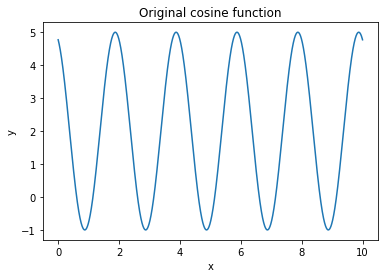
\includegraphics[width=.9\linewidth]{./obipy-resources/17087I4u.png}

Here it looks like we do have 5 periods in every interval of 10.
First we'll find these coefficients analytically in Mathematica: 

$$\text{args}=\left\{A\to 3,C\to 2,\varphi \to \frac{\pi }{8}\right\};$$
$$\text{hk}(\text{k$\_$},\text{h$\_$})\text{:=}\frac{1}{10} \int_0^{10} h(x)
e^{\frac{2}{10} \pi i k x} \, dx$$


$$h(\text{x$\_$})\text{:=}A \cos \left(\varphi +\frac{2\ 5 \pi  x}{10}\right)+C$$

$$\text{coefs}=\left| \text{Table}[N[\text{hk}(a,h)\text{/.}\,
\text{args}],\{a,-10,10\}]\right|$$

$$\{0.,0.,0.,0.,0.,1.5,0.,0.,0.,0.,2.,0.,0.,0.,0.,1.5,0.,0.,0.,0.,0.\}$$

So here, it looks like we only get coefficients at frequencies of $\frac{1}{2},
-\frac{1}{2}$, and $0$, with magnitudes of 1.5, 1.5, and 2.

Now let's check these values with numpy's fft:

\begin{minted}[frame=lines,fontsize=\scriptsize]{python}
def fft_and_freq(Y, d):
    fft = np.fft.fft(Y) / len(Y)
    freqs = np.fft.fftfreq(len(Y), d)
    return fft, freqs

def ifft(fftY, l):
    return np.fft.ifft(fftY * l)
\end{minted}


\begin{minted}[frame=lines,fontsize=\scriptsize]{python}
cosfft, cosfreqs = fft_and_freq(Y, (X[1] - X[0]))
\end{minted}


\begin{minted}[frame=lines,fontsize=\scriptsize]{python}
plt.plot(cosfreqs, np.abs(cosfft), '.')
plt.xlim([-1, 1])
plt.xlabel('Frequency')
plt.ylabel('Fft Magnitude')
plt.title('Fourier Transformed Cosine Function')
plt.show()
\end{minted}

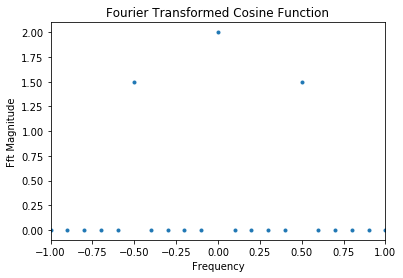
\includegraphics[width=.9\linewidth]{./obipy-resources/17087UWK.png}

\begin{minted}[frame=lines,fontsize=\scriptsize]{python}
plt.plot(X, ifft(cosfft, len(Y)))
plt.xlabel('x')
plt.ylabel('y')
plt.title('Inverse Transform of Cosine FFT')
plt.show()
\end{minted}

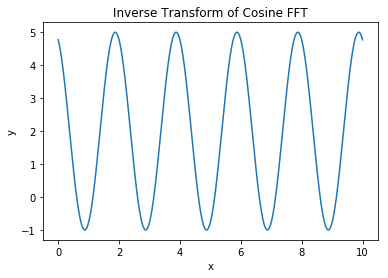
\includegraphics[width=.9\linewidth]{./obipy-resources/17087vd1.png}

Here the inverse again gives us the same thing we had before. Now let's do the
same thing for the Gaussian function:

\begin{minted}[frame=lines,fontsize=\scriptsize]{python}
def gaussian(t, A, B, L):
    return A * np.exp(-B * ((t - L / 2) ** 2))

# here we'll set A = 3, B = 2, L = 10
Xg = np.linspace(0, 10, 10000)
Yg = gaussian(Xg, 3., 2., 10.)
plt.plot(Xg, Yg)
plt.xlabel('t')
plt.ylabel('y')
plt.title('Original Gaussian Function')
plt.show()
\end{minted}

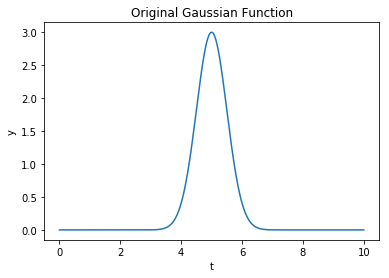
\includegraphics[width=.9\linewidth]{./obipy-resources/17087uqW.png}

\begin{minted}[frame=lines,fontsize=\scriptsize]{python}
gaussfft, gaussfreqs = fft_and_freq(Yg, (Xg[1] - Xg[0]))
plt.plot(gaussfreqs, np.abs(gaussfft), '.')
plt.xlim([-5, 5])
plt.xlabel('Frequency')
plt.ylabel('FFT Magnitude')
plt.title('Fourier Transformed Gaussian')
plt.show()
\end{minted}

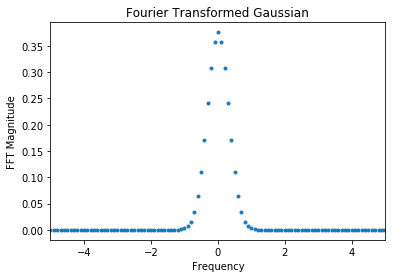
\includegraphics[width=.9\linewidth]{./obipy-resources/1708770c.png}

Here we do see that the Fourier transform of our Gaussian is indeed another
Gaussian.

\begin{minted}[frame=lines,fontsize=\scriptsize]{python}
plt.plot(Xg, ifft(gaussfft, len(Yg)))
plt.xlabel('x')
plt.ylabel('y')
plt.title('Inverse Transform of Gaussian FFT')
plt.show()
\end{minted}

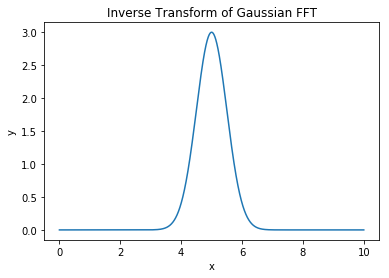
\includegraphics[width=.9\linewidth]{./obipy-resources/17087VJp.png}

So here we also find the inverse giving us the same function.

\section*{Part II}
\label{sec-2}

\subsection*{(1)}
\label{sec-2-1}

\begin{minted}[frame=lines,fontsize=\scriptsize]{python}
dataset1 = np.genfromtxt("/Users/tommyalford/Documents/Ph21/Set2/arecibo1.txt")
\end{minted}


\begin{minted}[frame=lines,fontsize=\scriptsize]{python}
plt.plot(dataset1)
plt.ylabel('Data')
plt.xlabel('Index (Time / .001 ms)')
plt.title('Arecibo1 Data')
plt.show()
\end{minted}

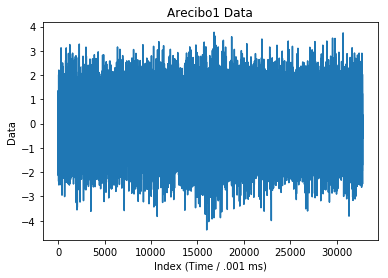
\includegraphics[width=.9\linewidth]{./obipy-resources/17087JHe.png}

Definitely looks pretty noisy here. Let's try ffting it.


\begin{minted}[frame=lines,fontsize=\scriptsize]{python}
set1fft, set1freqs = fft_and_freq(dataset1, d=.001)
\end{minted}


\begin{minted}[frame=lines,fontsize=\scriptsize]{python}
plt.plot(set1freqs, np.abs(set1fft))
plt.ylabel('FFT Magnitude')
plt.xlabel('Frequency')
plt.title('Transformed Arecibo1 Data')
plt.show()
\end{minted}

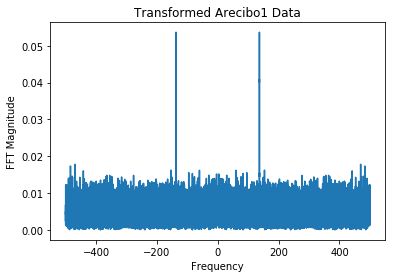
\includegraphics[width=.9\linewidth]{./obipy-resources/17087WRk.png}

Here we clearly see most of the signal near the frequency of 150Hz. Let's zoom
in on the data and then find this frequency more accurately:

\begin{minted}[frame=lines,fontsize=\scriptsize]{python}
plt.plot(set1freqs, np.abs(set1fft))
plt.xlim([130, 150])
plt.xlabel('Frequency')
plt.ylabel('FFT Magnitude')
plt.title('Fourier Transformed Arecibo1 Data')
plt.show()
\end{minted}

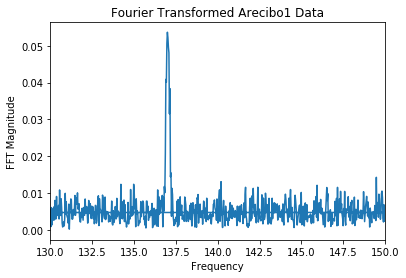
\includegraphics[width=.9\linewidth]{./obipy-resources/17087VQd.png}

\begin{minted}[frame=lines,fontsize=\scriptsize]{python}
set1freqs[np.argmax(np.abs(set1fft))]
\end{minted}

\begin{verbatim}
136.993408203125
\end{verbatim}


So, it looks like our signal has a frequency of 137 Hz!

\subsection*{(2)}
\label{sec-2-2}

\begin{minted}[frame=lines,fontsize=\scriptsize]{python}
def gaussian_envelope(t, t0, deltat):
    return np.exp((-(t - t0) ** 2) / (2 * deltat) ** 2)

def perfect_sin(t, f):
    return np.sin(2 * np.pi * f * t)

dt=.03
X = np.arange(-.1, .1, step=.001)
Y = perfect_sin(X, 137) * gaussian_envelope(X, 0, dt)

plt.plot(X, Y)
plt.title('Gaussian Envelope * Perfect Sinusoid')
plt.xlabel('x')
plt.ylabel('y')
plt.show()
\end{minted}

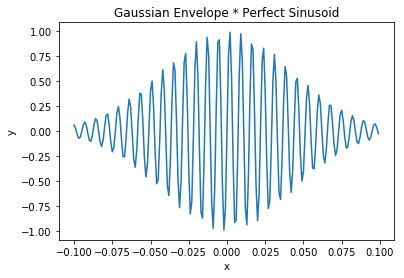
\includegraphics[width=.9\linewidth]{./obipy-resources/170877CF.png}

This looks right. Now we'll try Fourier transforming it to see what we get:

\begin{minted}[frame=lines,fontsize=\scriptsize]{python}
envfft, envfreqs = fft_and_freq(Y, d=.001)
\end{minted}


\begin{minted}[frame=lines,fontsize=\scriptsize]{python}
plt.plot(envfreqs, np.abs(envfft))
plt.title('Gaussian Envelope * Perfect Sinusoid, Transformed')
plt.xlabel('Frequency')
plt.ylabel('FFT Magnitude')
plt.show()
\end{minted}

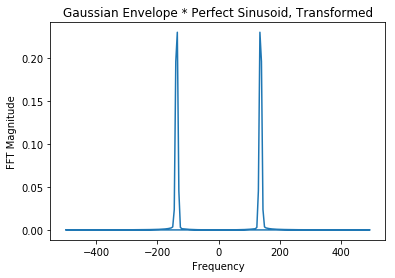
\includegraphics[width=.9\linewidth]{./obipy-resources/17087VXR.png}

Now we'll loop through a bunch of different $\Delta t$ values and plot
superimpose plots of them over the original fft data.

\begin{minted}[frame=lines,fontsize=\scriptsize]{python}
# need to normalize so that our max magnitude is the same as the first
# that way we can directly compare widths really
max_mag = np.max(np.abs(set1fft))
plt.figure(figsize=(10, 5))
plt.plot(set1freqs, np.abs(set1fft))
plt.xlim([133, 140])

X = np.arange(-10, 10, step=.001)
dtvals = [.001, .01, .1, 1]

def plot_envelope(dt):
    Yset = perfect_sin(X, 137) * gaussian_envelope(X, 0, dt)
    fft, freqs = fft_and_freq(Yset, d=.001)
    plt.plot(freqs, np.abs(fft) * (max_mag / np.max(np.abs(fft))), label=dt)

for dt in dtvals:
    plot_envelope(dt)

plt.legend()
plt.title('Gaussian Envlopes of Varying dt, Arecibo1 Data in Frequency Domain') 
plt.xlabel('Frequency (Hz)')
plt.xlabel('FFT Magnitude')
plt.show()
\end{minted}

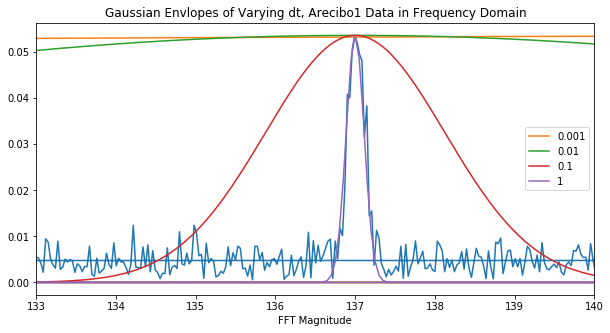
\includegraphics[width=.9\linewidth]{./obipy-resources/17087JAq.png}

Looks like $\Delta t = 1$ actually gives us a pretty close approximation. We
can try some more values near that:

\begin{minted}[frame=lines,fontsize=\scriptsize]{python}
plt.figure(figsize=(10, 5))
plt.plot(set1freqs, np.abs(set1fft))
plt.xlim([133, 140])
for dt in [.5, .75, 1, 1.25, 1.5]:
    plot_envelope(dt)

plt.legend()
plt.title('More Precise Gaussian Envlopes of Varying dt, Arecibo1 Data '
          'in Frequency Domain') 
plt.xlabel('Frequency (Hz)')
plt.xlabel('FFT Magnitude')
plt.xlim([136.5, 137.5])
plt.show()
\end{minted}

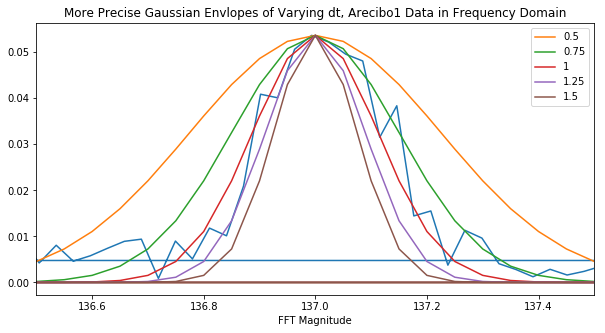
\includegraphics[width=.9\linewidth]{./obipy-resources/17087jU2.png}

This is pretty hard to tell at this point. Seems to be pretty close
to 1. Fitting using a real fit would be much more convienient.

\subsection*{(4)}
\label{sec-2-3}

\section*{Part III}
\label{sec-3}

\subsection*{(1)}
\label{sec-3-1}

We'll be trying out the scipy lombscargle algorithm.

\subsection*{(2)}
\label{sec-3-2}
\subsubsection*{Gaussian}
\label{sec-3-2-1}

\begin{minted}[frame=lines,fontsize=\scriptsize]{python}
# from before, we had Xg, Yg. Will take similar freqs here
lomb_freqs = np.linspace(-5, 5, 1000)
gausslomb = lombscargle(Xg, Yg, lomb_freqs)
\end{minted}


\begin{minted}[frame=lines,fontsize=\scriptsize]{python}
plt.plot(lomb_freqs, np.abs(gausslomb))
plt.xlabel('Frequency')
plt.ylabel('Lomb-Scargel Coefficients')
plt.title('Lomb-Scargle Transformed Gaussian Data')
plt.show()
\end{minted}

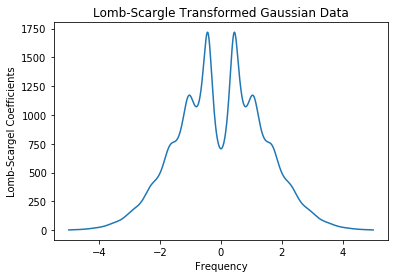
\includegraphics[width=.9\linewidth]{./obipy-resources/17087VeF.png}

\subsubsection*{Part II Data}
\label{sec-3-2-2}

\begin{minted}[frame=lines,fontsize=\scriptsize]{python}
set1_lomb_freqs = np.linspace(.1, 200, 10000)
set1_times = np.arange(len(dataset1) * .001, step=.001)
set1_lomb = lombscargle(set1_times, dataset1, set1_lomb_freqs)
\end{minted}


\begin{minted}[frame=lines,fontsize=\scriptsize]{python}
plt.plot(set1_lomb_freqs, np.abs(set1_lomb))
plt.xlabel('Frequency')
plt.ylabel('Lomb-Scargle Coefficients')
plt.title('Lomb-Scargle Transformed Arecibo1 Data')
plt.show()
\end{minted}

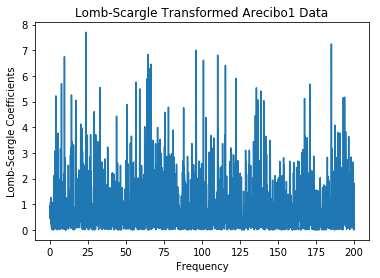
\includegraphics[width=.9\linewidth]{./obipy-resources/17087vyR.png}

Looks like it's a lot harder to find this signal now..

\subsection*{3}
\label{sec-3-3}
\begin{minted}[frame=lines,fontsize=\scriptsize]{python}
votable = parse("/Users/tommyalford/Documents/Ph21/set1/result_web_fileDR8owK.vot", 
                pedantic=False)
vo_data = votable.get_first_table().to_table()
\end{minted}


\begin{minted}[frame=lines,fontsize=\scriptsize]{python}
def plot_mag_data(mags, magerrs, MJDs):
    plt.figure(figsize=(12, 5))
    plt.errorbar(MJDs, mags, color='black', yerr=magerrs, fmt='o', markersize=3,
                ecolor='r', capthick=2)
    plt.gca().invert_yaxis()
    plt.xlabel('Date (MJD)')
    plt.ylabel('V mag')
\end{minted}


\begin{minted}[frame=lines,fontsize=\scriptsize]{python}
vo_mags = np.array(vo_data['Mag']).astype('float64')
vo_errs = np.array(vo_data['Magerr']).astype('float64')
vo_MJDs = np.array(vo_data['ObsTime']).astype('float64')
\end{minted}



\begin{minted}[frame=lines,fontsize=\scriptsize]{python}
vo_lomb_freqs = np.linspace(.1, 20, 10000)
vo_lomb = lombscargle(vo_mags.flatten(), vo_MJDs.flatten(), vo_lomb_freqs)
\end{minted}


\begin{minted}[frame=lines,fontsize=\scriptsize]{python}
plt.plot(vo_lomb_freqs, np.abs(vo_lomb), label='Lomb-Scargle Values')
plt.plot(1000 * [1.7], np.linspace(0, 6e11, 1000), '--', label='1.7 MJD')
plt.xlabel('Frequency')
plt.ylabel('Lomb-Scargle Coefficients')
plt.title('Lomb-Scargle Transformed Her X-1 Data')
plt.legend()
plt.show()
\end{minted}

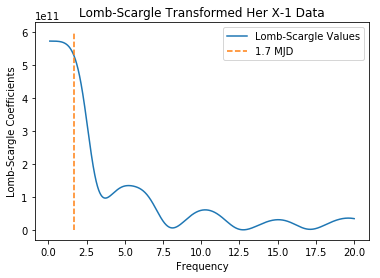
\includegraphics[width=.9\linewidth]{./obipy-resources/1708788X.png}

Here this might be the 1.7 MJD period that we want. Otherwise there are some
significant beats near 5, 10, 15 MJD
% Emacs 25.2.1 (Org mode 8.2.10)
\end{document}
